\documentclass[12pt]{article}
\usepackage[margin=2.5cm]{geometry}
\usepackage{enumerate}
\usepackage{amsfonts}
\usepackage{amsmath}
\usepackage{fancyhdr}
\usepackage{amsmath}
\usepackage{amssymb}
\usepackage{amsthm}
\usepackage{mdframed}
\usepackage{graphicx}
\usepackage{subcaption}
\usepackage{adjustbox}
\usepackage{listings}
\usepackage{xcolor}
\usepackage{booktabs}
\usepackage[utf]{kotex}

\definecolor{codegreen}{rgb}{0,0.6,0}
\definecolor{codegray}{rgb}{0.5,0.5,0.5}
\definecolor{codepurple}{rgb}{0.58,0,0.82}
\definecolor{backcolour}{rgb}{0.95,0.95,0.92}

\lstdefinestyle{mystyle}{
    backgroundcolor=\color{backcolour},
    commentstyle=\color{codegreen},
    keywordstyle=\color{magenta},
    numberstyle=\tiny\color{codegray},
    stringstyle=\color{codepurple},
    basicstyle=\ttfamily\footnotesize,
    breakatwhitespace=false,
    breaklines=true,
    captionpos=b,
    keepspaces=true,
    numbers=left,
    numbersep=5pt,
    showspaces=false,
    showstringspaces=false,
    showtabs=false,
    tabsize=1
}

\lstset{style=mystyle}

\pagestyle{fancy}
\renewcommand{\headrulewidth}{0.4pt}
\lhead{Hyungmo Gu}
\rhead{CSC209 Week 11 Notes}

\begin{document}
\title{CSC209 Week 11 Notes}
\author{Hyungmo Gu}
\maketitle

\section*{Processes 7 of 8}

\begin{itemize}
    \item Implementing the Shell Pipe Operator
    \begin{itemize}
        \item piping
        \begin{itemize}
            \item purpose is to send output from one end to input of anohter
            \item done by using \textit{dup2} and \textit{pipe}
            \item fd[0] and fd[1] must be closed after \textit{dup2}
        \end{itemize}
        \item dup2
        \begin{itemize}
            \item sets up redirection from fildes to fildes2
            \item \textbf{Syntax:} int dup2(int fildes, int fildes2)
            \begin{itemize}
                \item \textbf{fildes:} The source file descriptor
                \item \textbf{fildes2:} The destination file descriptor
            \end{itemize}
        \end{itemize}
        \item Example
        \begin{itemize}
            \item Executing \textit{sort} in parent and passing it to child for \textit{uniq}
            \begin{itemize}
                \item This is the same as `sort \textless file1 $\mid$ uniq'
            \end{itemize}

            \begin{center}
            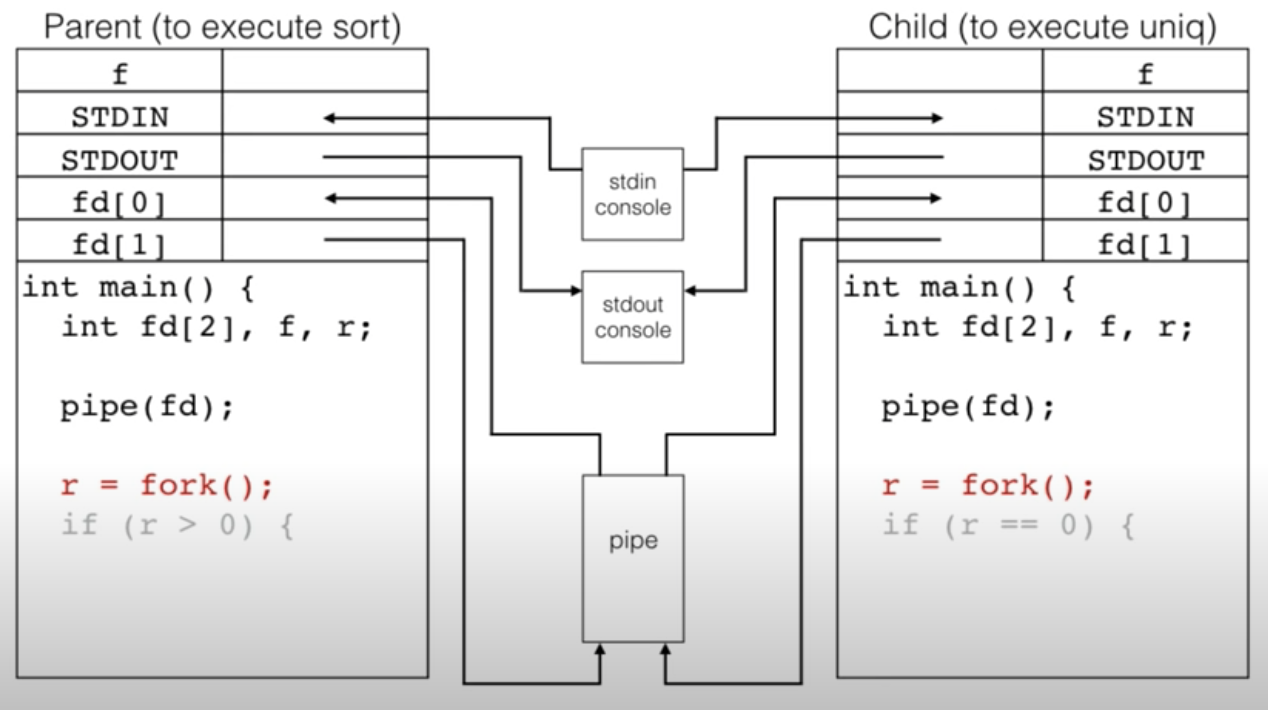
\includegraphics[width=\linewidth]{images/week_11_notes_1_1.png}
            
\includegraphics[width=\linewidth]{images/week_11_notes_1_2.png}
            \end{center}
        \end{itemize}

    \begin{lstlisting}[language=c, caption={pipe\_example\_1.c}]
    #include <stdio.h>
    #include <stdlib.h>
    #include <sys/types.h>
    #include <sys/stat.h>
    #include <fcntl.h>
    #include <unistd.h>
    #include <sys/wait.h>dd

    // equivalent to sort < file1 | uniq
    void sort_by_parent(int *fd);
    void uniq_by_child(int *fd);

    int main() {
        int fd[2], r;

        if ((pipe(fd) == -1)) {
            perror("pipe");
            exit(1);
        }

        r = fork();

        if (r < 0) {
            perror("fork");
            exit(1);
        }

        if (r > 0){
            sort_by_parent(fd);
        } else {
            uniq_by_child(fd);
        }
    }

    void sort_by_parent(int *fd) {
        int filedes = open("file1.txt", O_RDONLY);

        // reconfigure so all input from file1 are redirected to stdin
        if (dup2(filedes, fileno(stdin)) == -1) {
            perror("dup2.1");
            exit(1);
        }

        // reconfigure so all output from stdout is redirected to write part of pipe
        // this is to sent to uniq
        if (dup2(fd[1], fileno(stdout)) == -1) {
            perror("dup2.2");
            exit(1);
        }

        // close read part of pipe
        if (close(fd[0]) == -1) {
            perror("close1");
        }

        // close write since it's redirected to stdout
        if (close(fd[1]) == -1) {
            perror("close2");
        }

        // close file since it won't be used directly
        if (close(filedes) == -1) {
            perror("close3");
        }

        // executes terminal's sort
        execl("/usr/bin/sort", "sort", (char *) 0);
    }

    void uniq_by_child(int *fd) {
        // reconfigure stdin so that it reads from pipe
        if (dup2(fd[0], fileno(stdin))) {
            perror("dup2");
            exit(1);
        }
        // close the write pipe (see diagram)
        if (close(fd[1]) == -1) {
            perror("close");
        }

        // close the read pip since it will be read from stdin of pipe
        if (close(fd[0]) == -1) {
            perror("close");
        }

        execl("/usr/bin/uniq", "uniq", (char*) 0); // <- execute file from file path, and return 0 if successful
        fprintf(stderr, "ERROR: exec should not return\n"); // <- run if uniq not run
    }
    \end{lstlisting}

    \begin{lstlisting}[language=bash]
    >>> gcc -Wall pipe_example_1.c
    >>> ./a.out
    Fail T1
    Fail T2
    Fail T5
    Pass
    \end{lstlisting}

    \end{itemize}
\end{itemize}

\bigskip

\section*{}

\bigskip

\begin{itemize}
    \item \textbf{\&:} Allows the program to run simultaneously

    \begin{lstlisting}[language=bash]
    prog1 & prog2; #<- prog1 and prog2 runs in parallel
    prog1 & # <- prog1 runs in background, and cursor is returned immediately
    \end{lstlisting}

    \item \textbf{\#!:} Is PID of latest program that's running in the background

\end{itemize}

\end{document}